\section{Aim and Methodology}
The goal of this paper is to devise a general formula which accounts for certain parameters of the tree as well as the spacing between successive rotations of the garland to obtain the amount of the garland I would need to buy. To do so, I must first mathematically model the Christmas tree and the garland that wraps around the tree. This involves making some assumptions and approximations, in order to simplify the model:
\begin{wrapfigure}{r}{0.35\textwidth}
    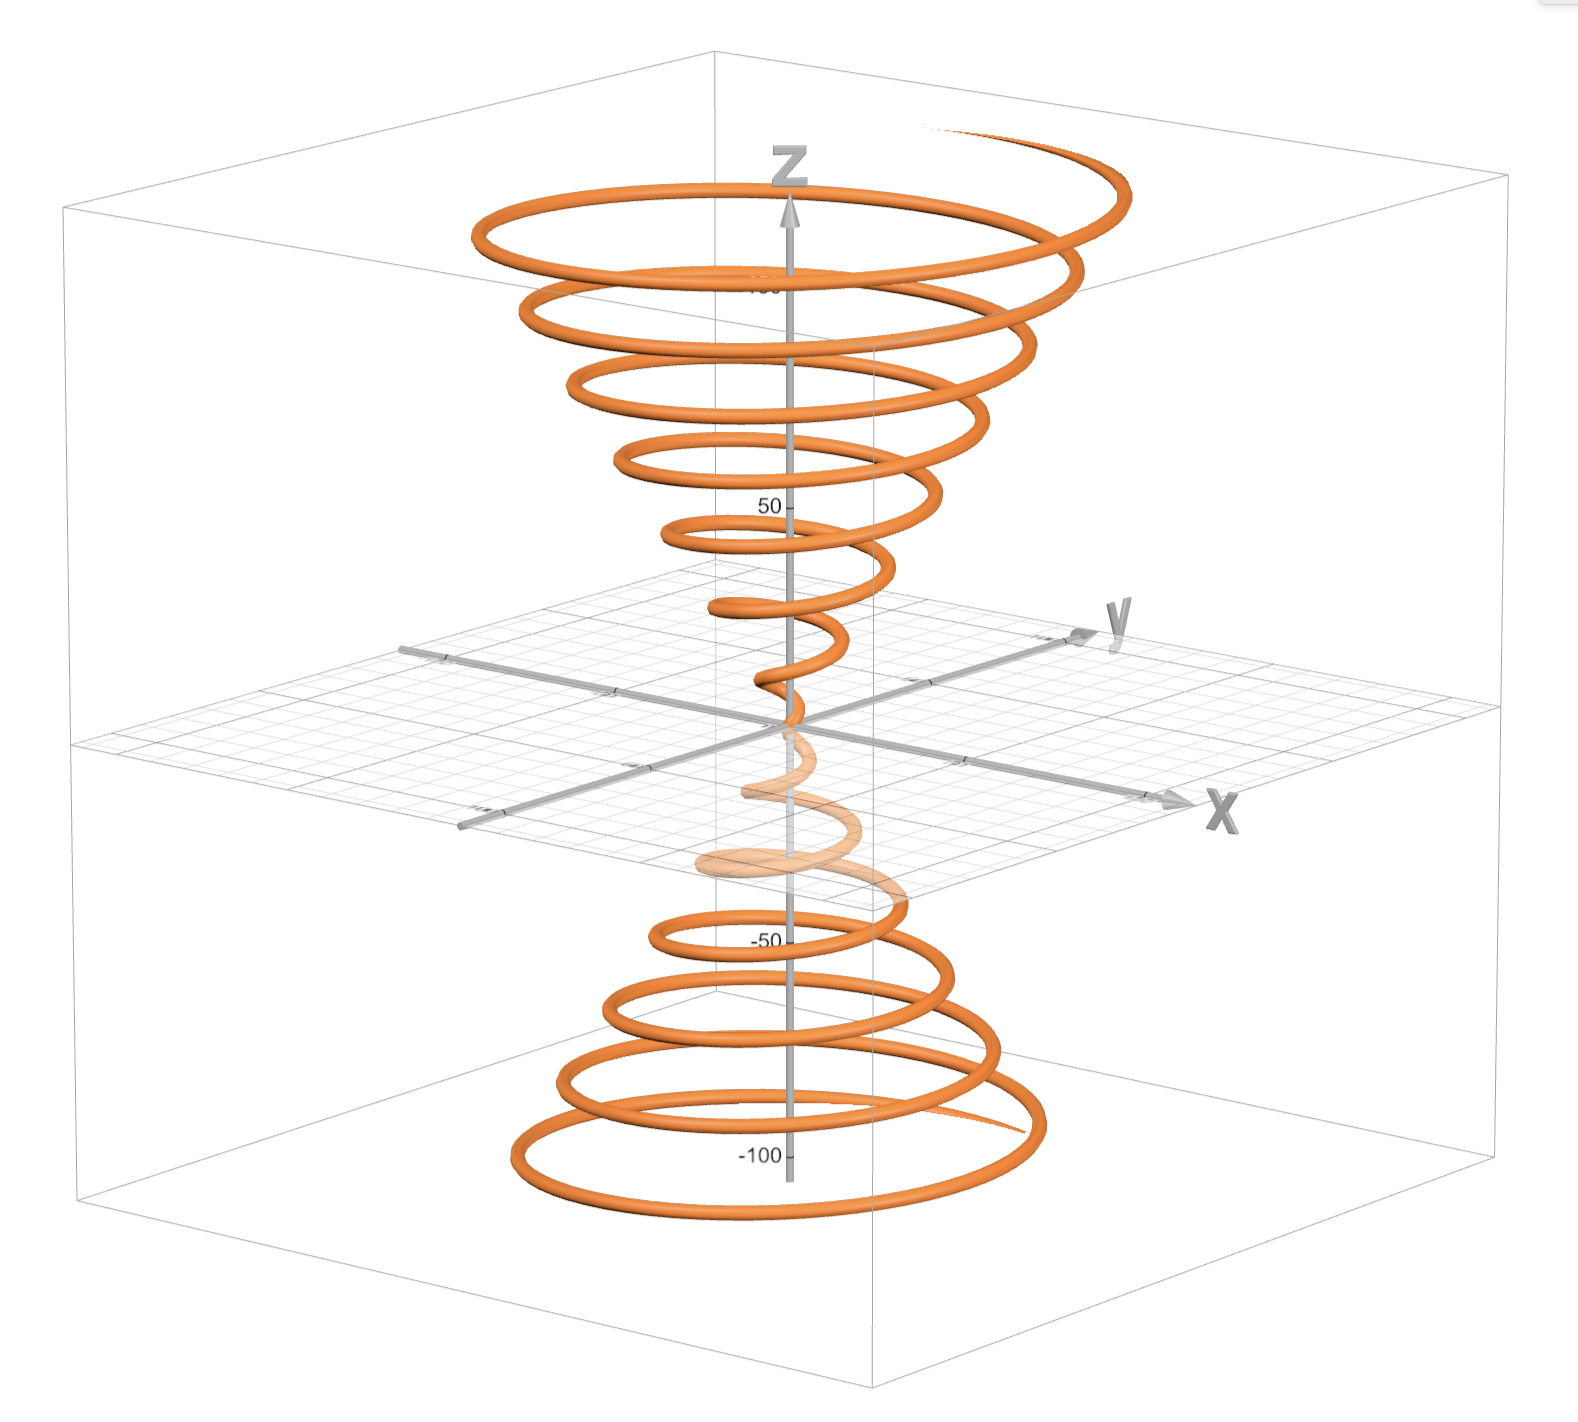
\includegraphics[width=0.32\textwidth]{images/unbounded_spiral.png}
    \caption{Unbounded Conical Spiral. (Generated using \emph{Desmos})}
    \vspace*{-20pt}
\end{wrapfigure}
\begin{enumerate}[leftmargin=!, itemindent=-5ex]
    \item \textbf{The Christmas tree is “ideal”} -- The Christmas tree is modelled as a \emph{cone}, based on the assumption that an “ideal” tree would be radially symmetrical all around and that the slant of the tree is a straight line.
    \item \textbf{The garland wraps uniformly} -- This means that it wraps in a perfect spiral around the tree, without sagging. The garland should also wrap around the tree with equal spacing between subsequent rotations. Since the tree is approximated to be a cone, the garland wrapping around the tree can be modelled as a \emph{circular conical spiral}.
\end{enumerate}
The following input parameters will be considered for the calculations (visualized in Figure \ref{fig:params}):

\noindent
\begin{minipage}{0.65\textwidth}
    \setlength{\parindent}{17pt}
    \begin{table}[H]
        \centering
        \singlespacing
        \begin{tabularx}{0.9\textwidth}{>{\hsize=0.4\hsize}c>{\hsize=0.6\hsize}X}
            \toprule
            {\bfseries Parameter} & {\bfseries Description}                                          \\
            \midrule
            $H$                   & height of the tree                                               \\
            $R$                   & radius of the based of the tree                                  \\
            $\lambda$             & slant distance (spacing) between successive rotations of garland \\
            \bottomrule
        \end{tabularx}
    \end{table}

    Diagrams and graphs will be used throughout the paper to aid in the explanation of concepts, and unless otherwise mentioned, all graphical visualizations are generated by myself using the online graphing calculator \emph{Desmos} and labelled using \emph{Adobe Illustrator}.
\end{minipage}
\begin{minipage}{0.35\textwidth}
    \centering
    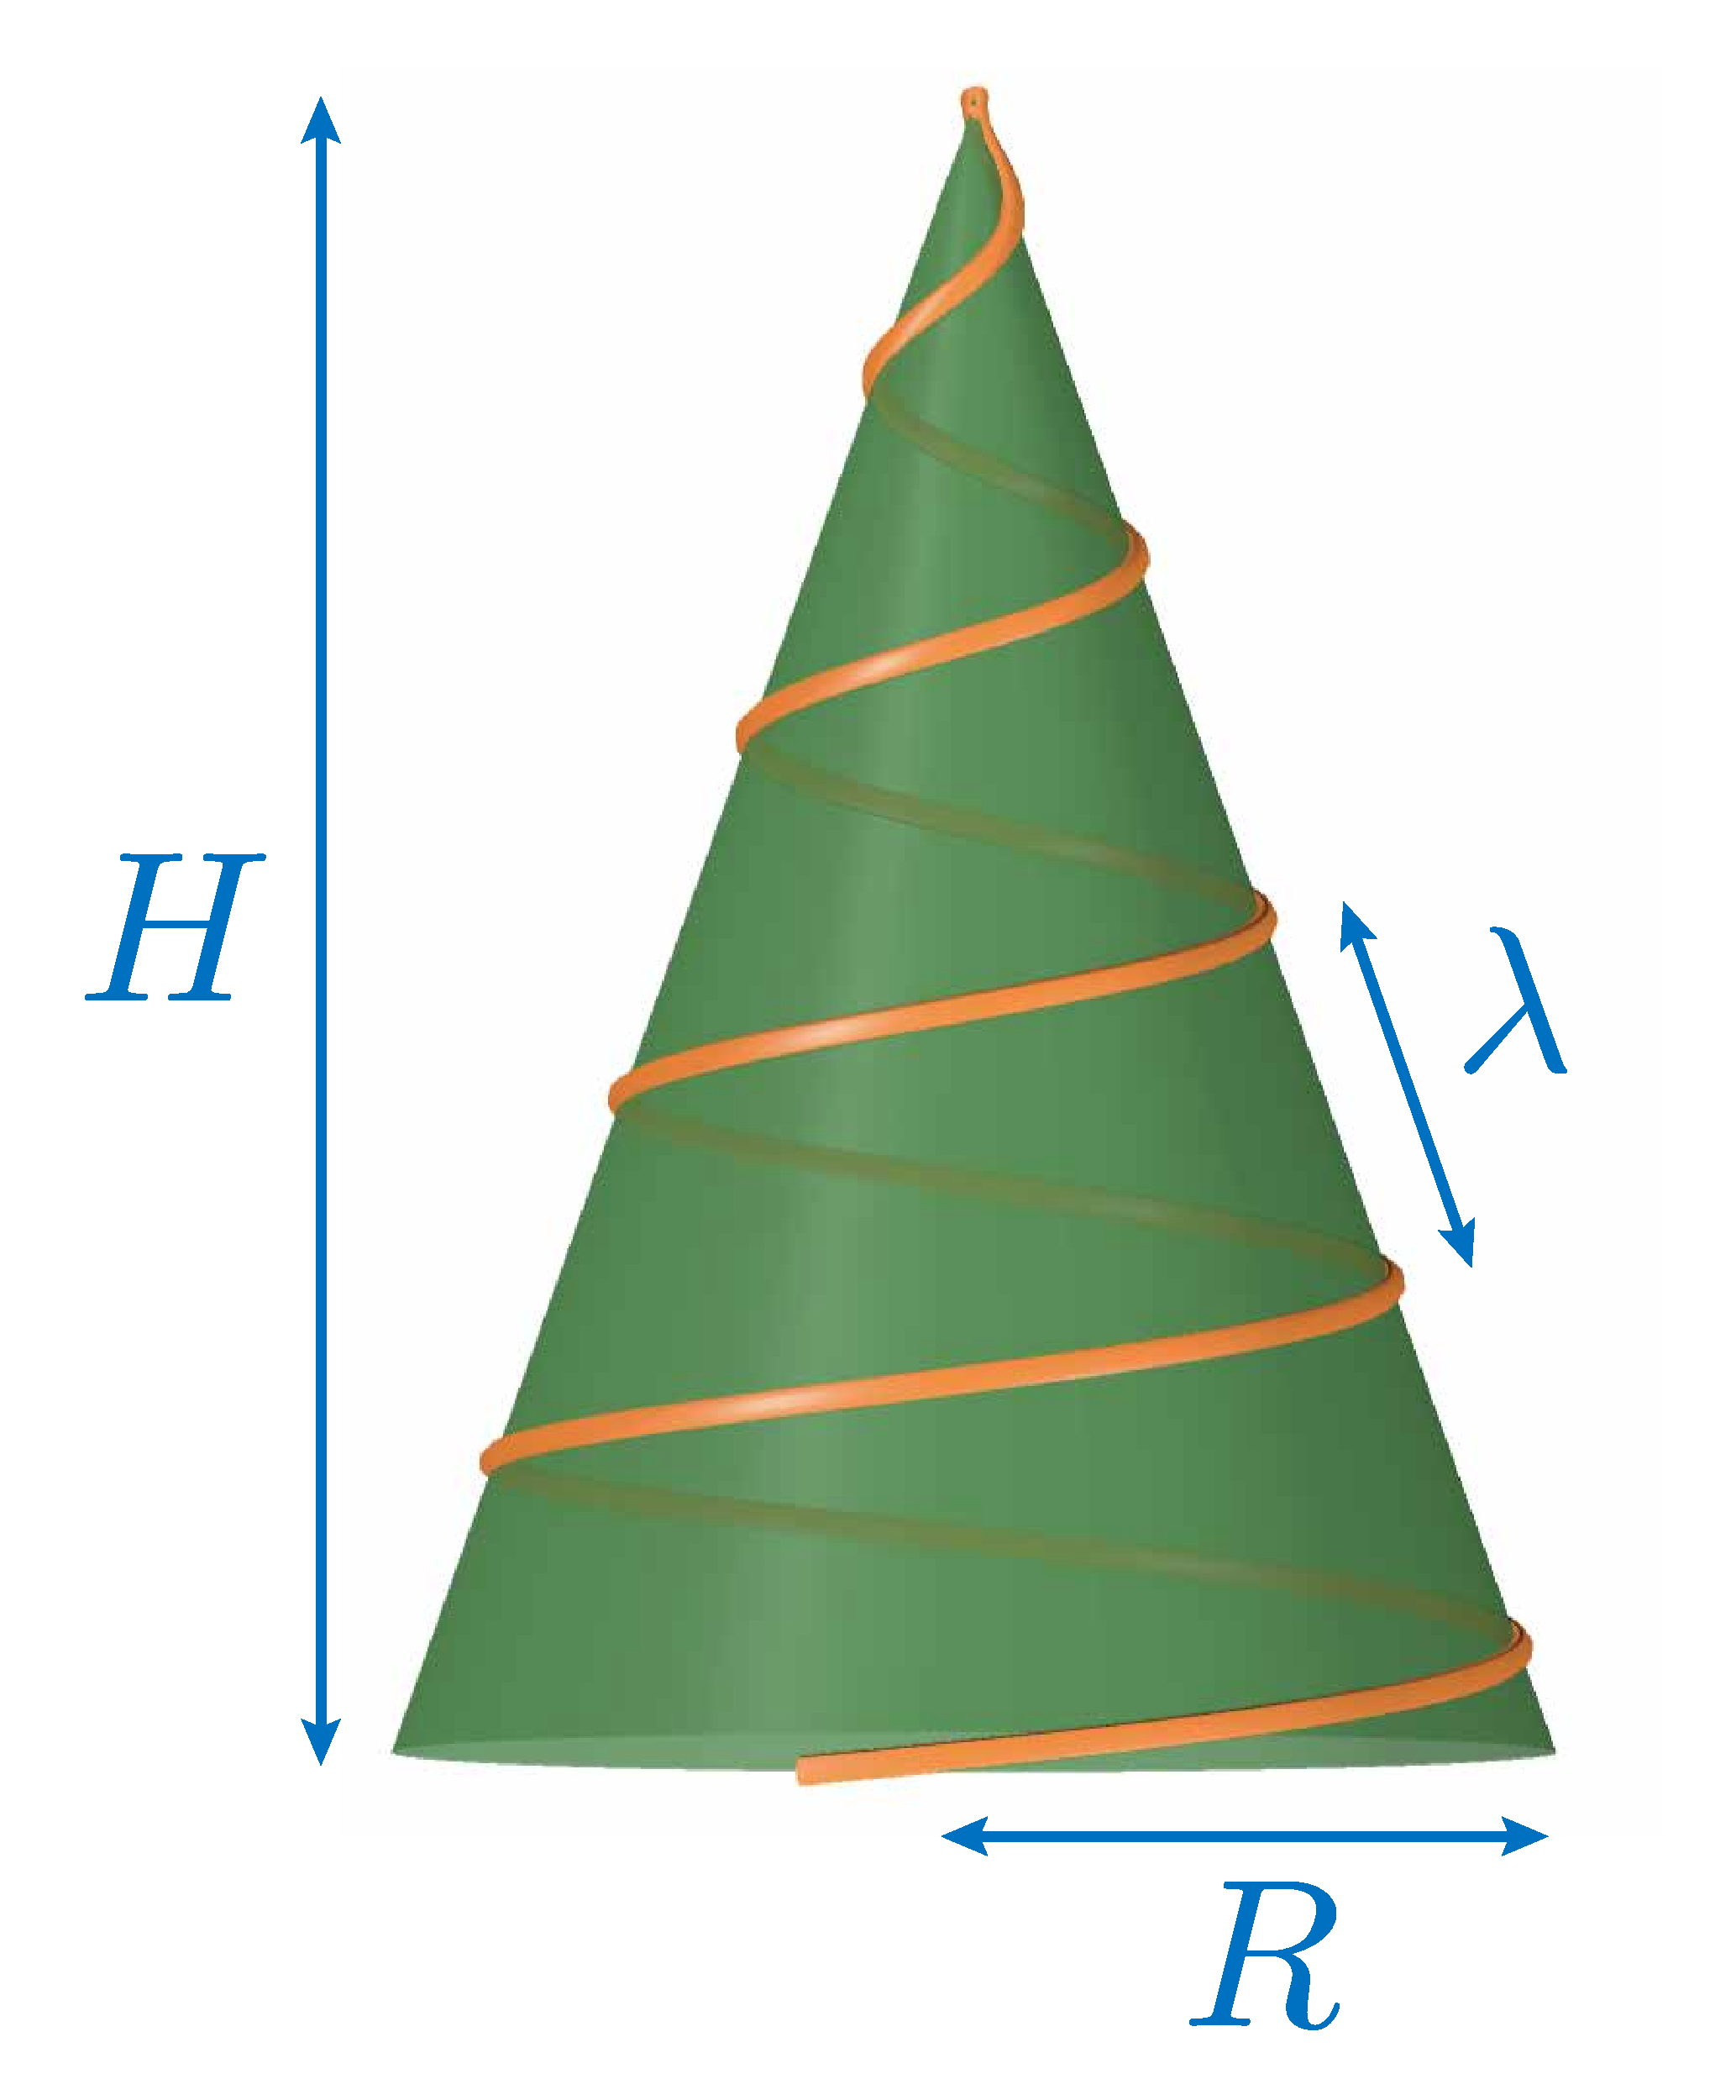
\includegraphics[width=0.85\textwidth]{diagrams/parameters.pdf}
    \captionof{figure}{Input Parameters.} \label{fig:params}
\end{minipage}


